% !TEX TS-program = pdflatex
% !TEX encoding = UTF-8 Unicode

%%%%%%%%%%%%%%%%%%%%%%%%%%%%%%%%%%%%%%%%%
% Structured General Purpose Assignment
% LaTeX Template
%
% This template has been downloaded from:
% http://www.latextemplates.com
%
% Original author:
% Ted Pavlic (http://www.tedpavlic.com)
%
% Note:
% The \lipsum[#] commands throughout this template generate dummy text
% to fill the template out. These commands should all be removed when 
% writing assignment content.
%
%%%%%%%%%%%%%%%%%%%%%%%%%%%%%%%%%%%%%%%%%

%----------------------------------------------------------------------------------------
%	PACKAGES AND OTHER DOCUMENT CONFIGURATIONS
%----------------------------------------------------------------------------------------

\documentclass[12pt]{article}
\usepackage[utf8]{inputenc} % set input encoding (not needed with XeLaTeX)

\usepackage{fancyhdr} % Required for custom headers
\usepackage{lastpage} % Required to determine the last page for the footer
\usepackage{extramarks} % Required for headers and footers
\usepackage{graphicx} % Required to insert images
\usepackage{caption}
\usepackage{float}
\usepackage{listings}
\usepackage{url}
\usepackage{subcaption}
\usepackage{amssymb}
\usepackage{textcomp}
\usepackage{color}
\usepackage[hidelinks]{hyperref}

\definecolor{lightgray}{rgb}{.9,.9,.9}
\definecolor{darkgray}{rgb}{.4,.4,.4}
\definecolor{purple}{rgb}{0.65, 0.12, 0.82}

\lstdefinelanguage{JavaScript}{
  keywords={typeof, new, true, false, catch, function, return, null, catch, switch, var, if, in, while, do, else, case, break},
  keywordstyle=\color{blue}\bfseries,
  ndkeywords={class, export, boolean, throw, implements, import, this},
  ndkeywordstyle=\color{darkgray}\bfseries,
  identifierstyle=\color{black},
  sensitive=false,
  comment=[l]{//},
  morecomment=[s]{/*}{*/},
  commentstyle=\color{purple}\ttfamily,
  stringstyle=\color{red}\ttfamily,
  morestring=[b]',
  morestring=[b]"
}

\lstset{
   language=JavaScript,
   backgroundcolor=\color{lightgray},
   extendedchars=true,
   basicstyle=\footnotesize\ttfamily,
   showstringspaces=false,
   showspaces=false,
   numbers=left,
   numberstyle=\footnotesize,
   numbersep=9pt,
   tabsize=2,
   breaklines=true,
   showtabs=false,
   captionpos=b
}

\hypersetup{colorlinks=false}

% Margins
\topmargin=-0.45in
\evensidemargin=0in
\oddsidemargin=0in
\textwidth=6.5in
\textheight=9.0in
\headsep=0.25in 


\linespread{1.1} % Line spacing

% Set up the header and footer
\pagestyle{fancy}
\lhead{\hmwkAuthorName} % Top left header
\chead{\hmwkClass\ \hmwkTitle} % Top center header
\rhead{\firstxmark} % Top right header
\lfoot{\lastxmark} % Bottom left footer
\cfoot{} % Bottom center footer
\rfoot{Page\ \thepage\ of\ \pageref{LastPage}} % Bottom right footer
\renewcommand\headrulewidth{0.4pt} % Size of the header rule
\renewcommand\footrulewidth{0.4pt} % Size of the footer rule

\setlength\parindent{0pt} % Removes all indentation from paragraphs

%----------------------------------------------------------------------------------------
%	DOCUMENT STRUCTURE COMMANDS
%	Skip this unless you know what you're doing
%----------------------------------------------------------------------------------------

% Header and footer for when a page split occurs within a problem environment
\newcommand{\enterProblemHeader}[1]{
\nobreak\extramarks{#1}{#1 continued on next page\ldots}\nobreak
\nobreak\extramarks{#1 (continued)}{#1 continued on next page\ldots}\nobreak
}

% Header and footer for when a page split occurs between problem environments
\newcommand{\exitProblemHeader}[1]{
\nobreak\extramarks{#1 (continued)}{#1 continued on next page\ldots}\nobreak
\nobreak\extramarks{#1}{}\nobreak
}

\setcounter{secnumdepth}{0} % Removes default section numbers
\newcounter{homeworkProblemCounter} % Creates a counter to keep track of the number of problems

\newcommand{\homeworkProblemName}{}
\newenvironment{homeworkProblem}[1][Problem \arabic{homeworkProblemCounter}]{ % Makes a new environment called homeworkProblem which takes 1 argument (custom name) but the default is "Problem #"
\stepcounter{homeworkProblemCounter} % Increase counter for number of problems
\renewcommand{\homeworkProblemName}{#1} % Assign \homeworkProblemName the name of the problem
\section{\homeworkProblemName} % Make a section in the document with the custom problem count
\enterProblemHeader{\homeworkProblemName} % Header and footer within the environment
}{
\exitProblemHeader{\homeworkProblemName} % Header and footer after the environment
}

\newcommand{\problemAnswer}[1]{ % Defines the problem answer command with the content as the only argument
\noindent\framebox[\columnwidth][c]{\begin{minipage}{0.98\columnwidth}#1\end{minipage}} % Makes the box around the problem answer and puts the content inside
}

\newcommand{\homeworkSectionName}{}
\newenvironment{homeworkSection}[1]{ % New environment for sections within homework problems, takes 1 argument - the name of the section
\renewcommand{\homeworkSectionName}{#1} % Assign \homeworkSectionName to the name of the section from the environment argument
\subsection{\homeworkSectionName} % Make a subsection with the custom name of the subsection
\enterProblemHeader{\homeworkProblemName\ [\homeworkSectionName]} % Header and footer within the environment
}{
\enterProblemHeader{\homeworkProblemName} % Header and footer after the environment
}
   
%----------------------------------------------------------------------------------------
%	NAME AND CLASS SECTION
%----------------------------------------------------------------------------------------

\newcommand{\hmwkTitle}{`Virtual Sun-Earth-Moon System'} % Assignment title
\newcommand{\hmwkDueDate}{Thursday,\ November\ 19,\ 2015} % Due date
\newcommand{\hmwkClass}{CS\ 32310} % Course/class
\newcommand{\hmwkAuthorName}{James Euesden - jee22} % Your name

%----------------------------------------------------------------------------------------
%	TITLE PAGE
%----------------------------------------------------------------------------------------

\title{
\vspace{2in}
\textmd{\textbf{\hmwkClass:\ \hmwkTitle}}\\
\normalsize\vspace{0.1in}\small{Due\ on\ \hmwkDueDate}\\
\vspace{3in}
}

\author{\textbf{\hmwkAuthorName}}
\date{} % Insert date here if you want it to appear below your name

%----------------------------------------------------------------------------------------

\setlength\parindent{24pt}

\begin{document}

\maketitle

%----------------------------------------------------------------------------------------
%	TABLE OF CONTENTS
%----------------------------------------------------------------------------------------

%\setcounter{tocdepth}{1} % Uncomment this line if you don't want subsections listed in the ToC

\newpage
\tableofcontents
\newpage

%----------------------------------------------------------------------------------------
%	INTRODUCTION
%----------------------------------------------------------------------------------------

% To have just one problem per page, simply put a \clearpage after each problem

\section{Introduction}
This assignment tasked me with using WebGL to create and display a simple animated model of the Sun-Earth-Moon system \cite{assignment}, requesting the basic features of display (three spheres with textures, orbits and rotations). There was also the option to implement additional functionality (lighting and shading, tilted axial and orbital rotations, etc). The model was not requested to be accurate in sizes, distances or times of rotations, although real world values were provided for reference.

%----------------------------------------------------------------------------------------
%	Basic Features
%----------------------------------------------------------------------------------------
\section{Simulation}
\subsection{Parameters}
In order to create the simple model, I used some arbitary values that made the system look somewhat accurate without truly being accurate. This was necessary in order for a viewer to see much of anything, as real values would leave the Sun too large compared to a miniscule Earth and Moon that would also be very, very far away from the camera focus. With the changing of the scale of the Earth and Moon for display purposes and the assignment requesting a simple simulation, I took liberties to use values that looked good for the simulation while not impacting the main aspects of it (rotations, spinning on axes, orbital and axial tilts, etc). These parameters are:

\begin{lstlisting}
// Large, so we can actually see something with our model.
var eccentricityModifier = 50; 
// For Elliptical orbits/Kepler's 2nd Law. Number of steps for an orbit.
var orbitSteps = 1000;

var earthSize = 10; // from -> 1 * 10; 
var earthDistanceFromSun = 156; // from -> 23500 / 150; 
var earthOrbitRotationSpeed = 0.089; // from -> 365.26 / 4000; 
var earthAxisRotationSpeed= 4.5; // from -> 9.972 / 2; 
var earthAxialTilt = 23.44;
var earthOrbitEccentricity = 0.00167 * eccentricityModifier;

var moonSize = 6; // from -> 0.277 * 21;
var moonDistanceFromEarth = 40; // from -> 60.3 / 1.5
var moonAxisRotationSpeed = 1.2; // from -> 2.732 / 2.4;
// var moonOrbitRotationSpeed=moonAxisRotationSpeed; // No Longer needed!
var moonOrbitEccentricity = 0.00549 * eccentricityModifier;
var moonAxialTilt = 1.593;
var moonOrbitalTilt = 5.145;

var sunSize = 20; // from -> 109 / 7;
var sunAxisRotationSpeed = 0.05; // from -> 0.25 / 4;

var starMapSize = 500;
\end{lstlisting}

As you can see, the Sun is much smaller than it should be, as are the distances between the Sun, Earth and Moon. I felt these numbers gave a good representation for this model, but should not be used if the model were intended to be an accurate representation of the system.

\subsection{Structure}
I have structured my JavaScript code such that there are files for each major component of the model (user interface, Sun-Earth-Moon in one file, Controller, etc) that handles the responsibilty of those components, for initiation and updating on each animation loop. Fror the Sun, Earth and Moon, each is held in their own object, which contains data of their Mesh, a constant reference to their homogeneous coordinates and their update methods.

Most of the values that parameters for controlling speed, size and the tilts of the planets are contained in a single global variable file, for easy access when I was building and testing my simulation. The setup and main rendering loop are in a single Controller file, and this calls to methods in the other files in the order that things should be initialised and updated. This made it easier to ensure the correct ordering of events.

The Earth and Moon mesh objects have also been added into one single Object3D, earthAndMoon, and then that object has been added to the scene, instead of adding the two individually. This increases the efficiency of the rendering, as they are rendered as one item. While not necessary for such a small simulation, if the application were expanded upon in the future to include many, maybe thousands, of additional planets, this style of structure would be much easier to maintain. It would also help group planets and their moons together, meaning they could be added and removed with their satellites easily.

\subsection{Running the program}
To run the simulation for demonstation, visit: \url{http://users.aber.ac.uk/jee22/cs323/virtual-system/}, hosted on my university filestore. For building and testing, I ran the application locally using xampp\cite{xampp} . You should be able to see the application in full working order in both B59 and C56, best seen in Firefox browser. No additional downloading is required. There is also a Credits page any textures and code used in the application here: \url{http://users.aber.ac.uk/jee22/cs323/virtual-system/credits.html}.


%----------------------------------------------------------------------------------------
%	Basic Features
%----------------------------------------------------------------------------------------

\section{Basic Features}
\subsection{The earth orbits the centre of the Sun}
The Earth has a clear orbit around the centre of the Sun, although it is an elliptical orbit and so may look a little off centre in the screenshot. If you view the images below, you can see how the orbit is set up around the Sun. This is achieved through pre-computed points of the orbital rotation using Kepler's 2nd Law of planetary motion (more on this in Additional Features section), which generates an elliptical orbit with varying speeds depending on the point of orbit.

\begin{figure}[H]
        \centering
        \begin{subfigure}[b]{0.4\textwidth}
                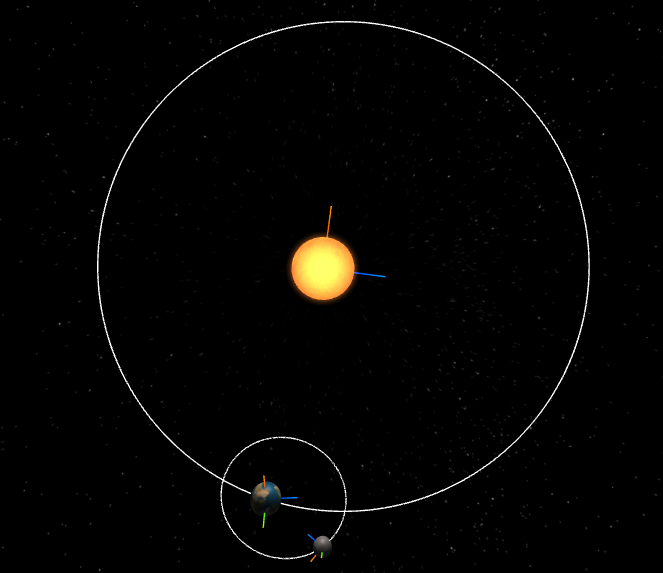
\includegraphics[width=\textwidth]{images/earthorbitsun1}
                \caption{View from above.}
                \label{fig: The Earth orbiting the Sun}
       \end{subfigure}
       %add desired spacing between images, e. g. ~, \quad, \qquad etc.
         %(or a blank line to force the subfigure onto a new line)
        \begin{subfigure}[b]{0.4\textwidth}
                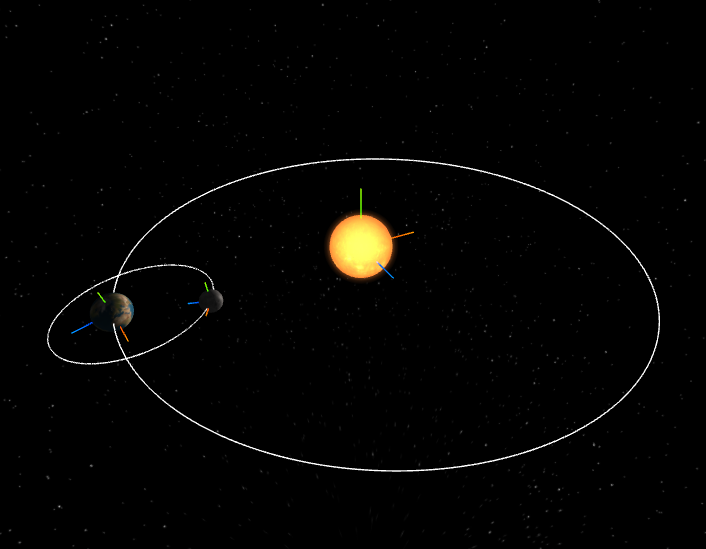
\includegraphics[width=\textwidth]{images/earthorbitsun2}
                \caption{View from the side.}
                \label{fig:The Earth orbiting the Sun}
       \end{subfigure}
       \caption{Views of the Earth's Orbit around the centre of the Sun (elliptical), shown by the orbit lines.}\label{fig: The Earth orbitng the centre of the Sun}
\end{figure}

Originally, the Earth orbited the Sun through updating the x and z coordinates, each animation frame updating the new position of the Earth by shifting it a certain amount, using the distance from the Sun, the speed of rotation the current x and z position and using radians to create the next step on the full anti-clockwise orbit.

\subsection{The moon orbits the centre of the Earth}
The Moon orbits the centre of the Earth in much the same way that the Earth orbits the Sun. The points are pre-computed, yet take into account the Earth's current position too. The orbit is ellipitcal, and as in reality, doesn't sit squarely 'centrally circling' the Earth. More information can be found out about this later in the report.

\begin{figure}[H]
        \centering
        \begin{subfigure}[b]{0.4\textwidth}
                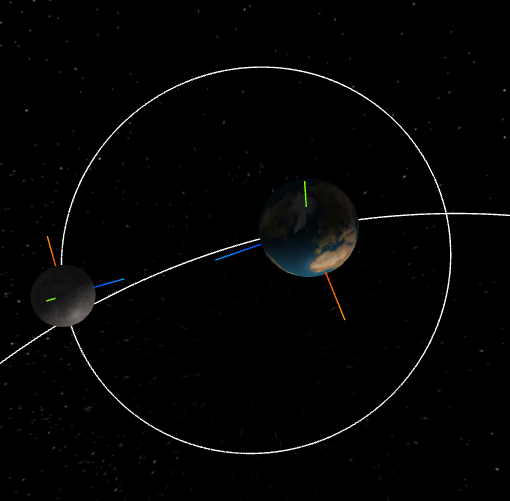
\includegraphics[width=\textwidth]{images/moonorbitearth1}
                \caption{View from above.}
                \label{fig: The Moon orbiting the Earth.}
       \end{subfigure}
       %add desired spacing between images, e. g. ~, \quad, \qquad etc.
         %(or a blank line to force the subfigure onto a new line)
        \begin{subfigure}[b]{0.4\textwidth}
                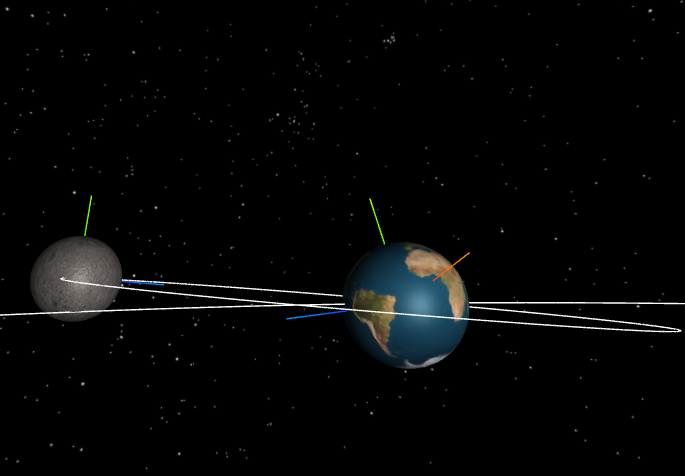
\includegraphics[width=\textwidth]{images/moonorbitearth2}
                \caption{View from the side.}
                \label{fig:The Earth orbiting the Sun}
       \end{subfigure}
       \caption{Views of the Moon's Orbit around the centre of the Earth (elliptical), shown by the orbit lines.}\label{fig: The Moon orbitng the centre of the Earth}
\end{figure}

\subsection{Circular orbits}
When I first built the simulation, the orbits were completely circular, but for a challenge I made them Elliptical, you can see Additional Features for more information. When they were circular though, they were done like this: 

\begin{lstlisting}
function updateOrbit(objectToUpdate, pivotPosition, orbitDistanceFromPivot, orbitAngleThisStep){
     objectToUpdate.position.x = pivotPosition.x + (orbitDistanceFromPivot * -Math.cos(orbitAngleThisStep));
     objectToUpdate.position.z = pivotPosition.z + (orbitDistanceFromPivot * -Math.sin(orbitAngleThisStep));
 }
 \end{lstlisting}
Where objectToUpdate was the Earth or Moon, pivotPosition the centre of the orbit, orbitDistanceFromPivot the distance between the centre of orbit and the object to orbit and the orbitAngleThisStep being the angle of rotation for the next position for the object to move, in radians.
 
If I were to do this in matrix transformations, I would do a similar process to updating the x and z position, but rather than updating them with .x and .z =, I would turn the coordinates into a homogeneous matrix and then multiply a shift on the x matrix and z matrix transformations together, apply that to the homogeneous coordinates, then convert them back to physical coordinates, update the object's vertices with its new position and then update the face and vertex normals with the normal of the transformation matrix. 
 
Doing this is not necessary for the orbital rotations as they are pre-computed. I have, however, done this for axial rotations and this can be seen in the subsection for the Sun, Earth and Moon spinning on their own axes.

\subsection{The Sun, Earth and Moon shown as texture mapped spheres}
As shown below, each object has it's own texture mapped to the surface. As an addition to this, the Earth and Moon have bump maps which make it look like their surfaces are not completely smooth, as in reality. The Earth additionally has a specular map, which allows the light from the Phong lighting and shading to reflect off of the reflective water of the Earth but not so much the land masses. The textures for the Earth and Moon come from planetpixel \cite{earthtextures}, while the Sun texture is credited to NASA\cite{suntexture}

\begin{figure}[H]
        \centering
        \begin{subfigure}[b]{0.4\textwidth}
                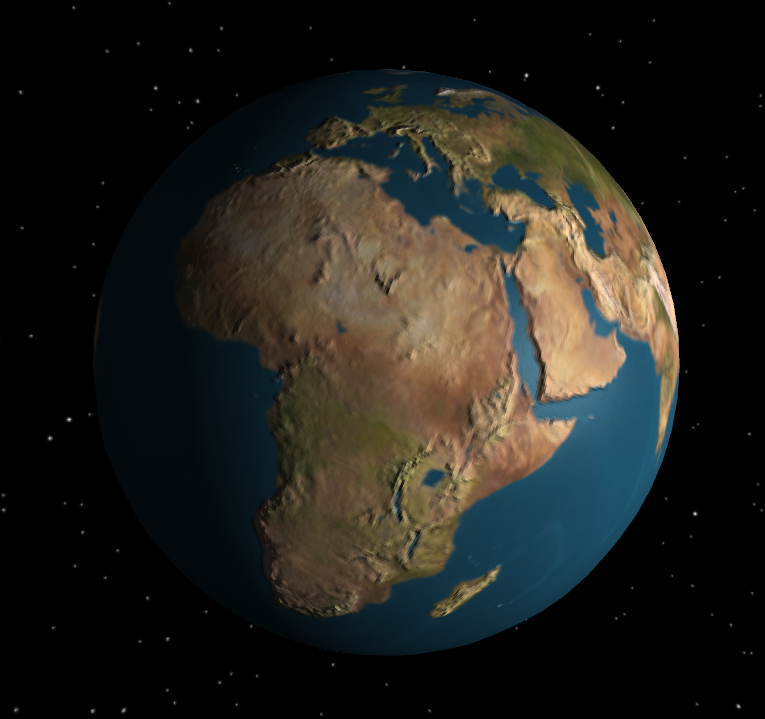
\includegraphics[width=\textwidth]{images/earthtexture}
                \caption{Earth texture maps}
                \label{fig: The Earth texture mapped.}
       \end{subfigure}
       %add desired spacing between images, e. g. ~, \quad, \qquad etc.
         %(or a blank line to force the subfigure onto a new line)
                 \begin{subfigure}[b]{0.4\textwidth}
                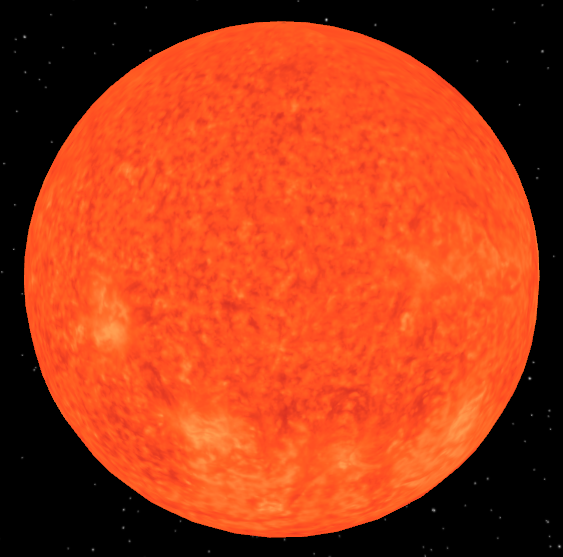
\includegraphics[width=\textwidth]{images/suntexture}
                \caption{Sun texture map}
                \label{fig: The Sun texture mapped}
       \end{subfigure}
        \begin{subfigure}[b]{0.4\textwidth}
                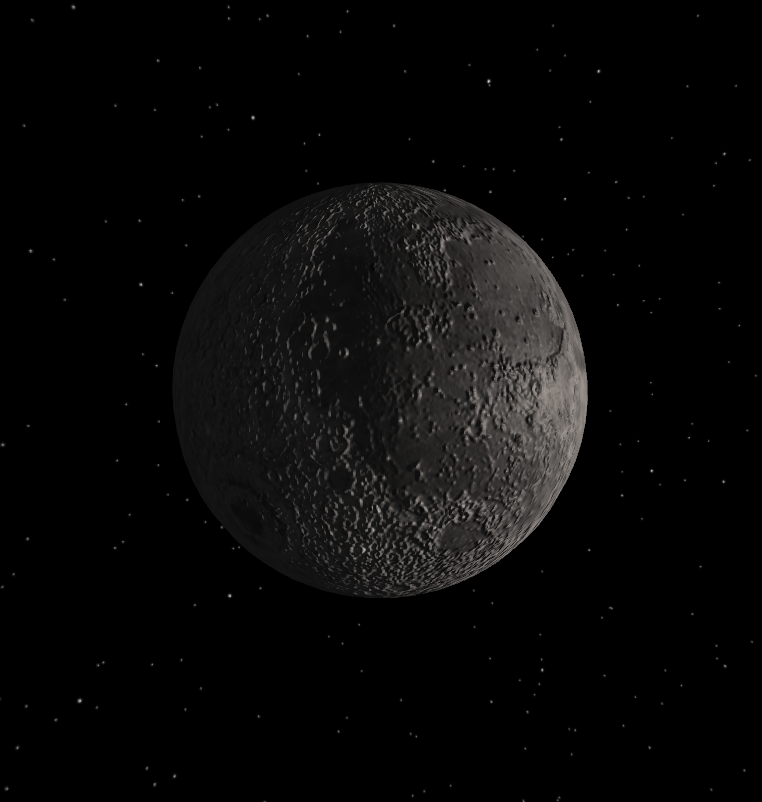
\includegraphics[width=\textwidth]{images/moontexture}
                \caption{Moon texture maps}
                \label{fig: The Moon texture mapped}
       \end{subfigure}
       \caption{The objects of the simulation, texture mapped to look like the planets they represent.}\label{fig: Texture mapped Sun, Earth and Moon.}
\end{figure}

\subsection{The Sun, Earth and Moon each spinning on their own axes}
They do, here, look at this picture of the Axis Helper showing that they're spinning on their axes. they do this through matrix transformation of rotation, as can be seen here: We turn Object geometry vertices into homogeneous coordinates (unnecessary for rotation, but for the sake of allowing for future adaptations that may wish to use translate transformations that need the 'w' coordinate too, we do this), multiply by the rotation this step (which is multiplied by the speed of the objects rotation) and then applied back to the Object geometries coordinates. Rotation!

While difficult to show in just images, you can see from the figure below that the Earth spins on it's own axis.
\begin{figure}[H]
        \centering
        \begin{subfigure}[b]{0.4\textwidth}
                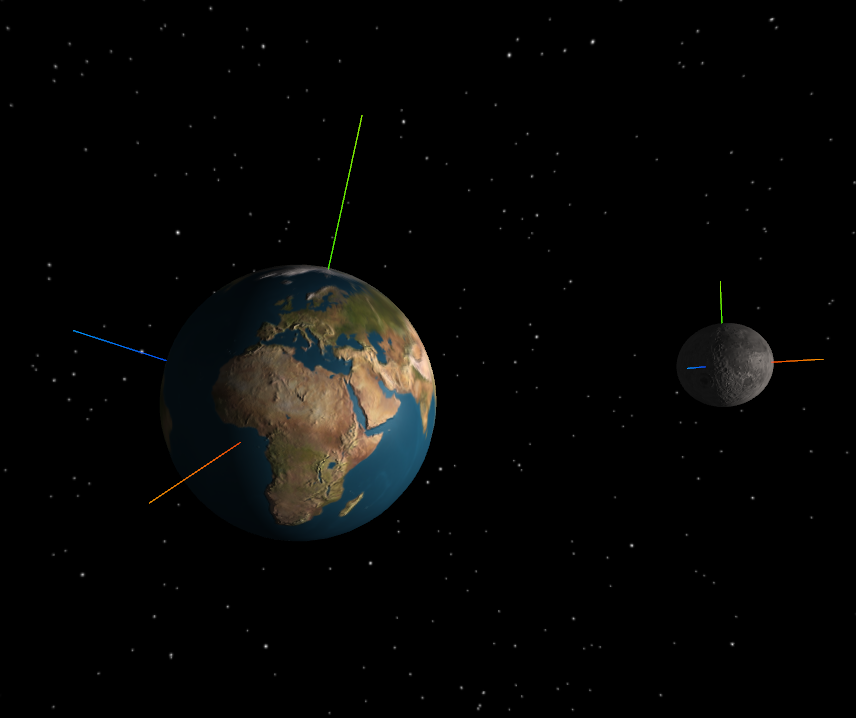
\includegraphics[width=\textwidth]{images/earthandmoonaxisspin1}
                \caption{The Earth and Moon spinning on their own axes}
                \label{fig: The axial spin of the Earth and moon.}
       \end{subfigure}
        \begin{subfigure}[b]{0.4\textwidth}
                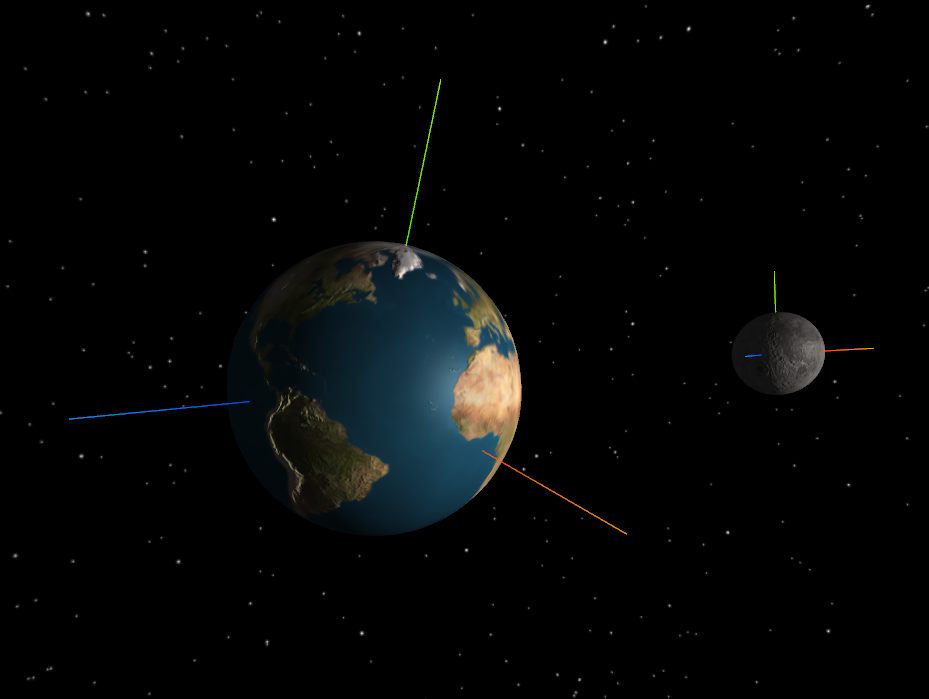
\includegraphics[width=\textwidth]{images/earthandmoonaxisspin2}
                \caption{The Earth and Moon spinning on their own axes}
                \label{fig: The axial spin of the Earth and moon.}
       \end{subfigure}
               \begin{subfigure}[b]{0.4\textwidth}
                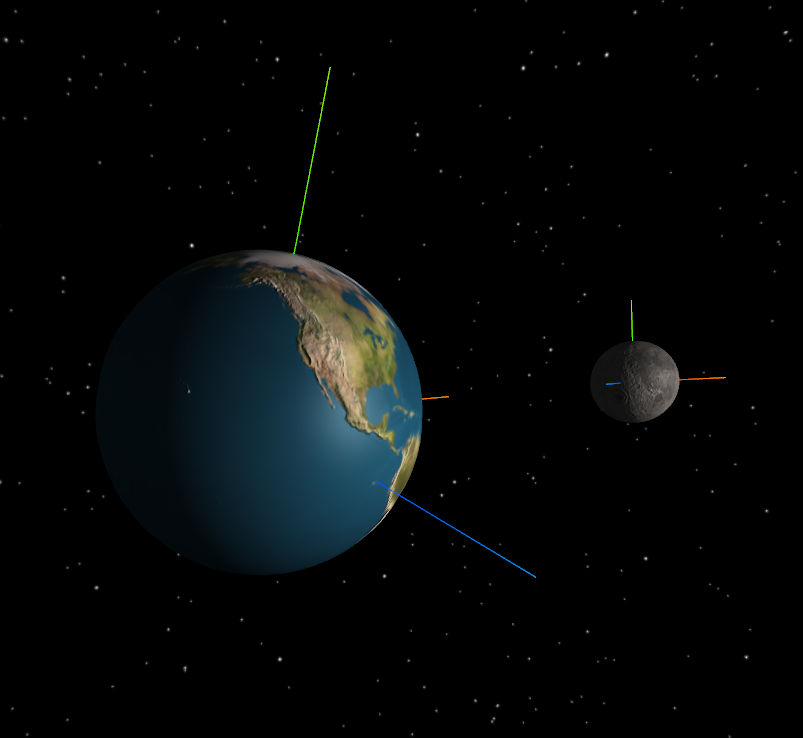
\includegraphics[width=\textwidth]{images/earthandmoonaxisspin3}
                \caption{The Earth and Moon spinning on their own axes}
                \label{fig: The axial spin of the Earth and moon.}
       \end{subfigure}
               \begin{subfigure}[b]{0.4\textwidth}
                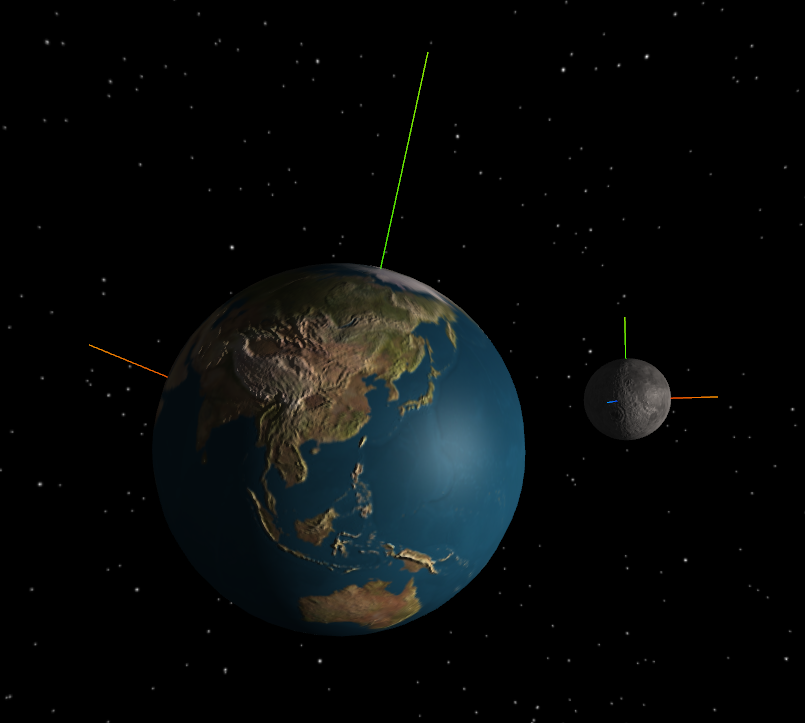
\includegraphics[width=\textwidth]{images/earthandmoonaxisspin4}
                \caption{The Earth and Moon spinning on their own axes}
                \label{fig: The axial spin of the Earth and moon.}
       \end{subfigure}
       \caption{Collections of images to present the Earth spinning on its own axis.}\label{fig: The Earth's individual rotation.}
\end{figure}

To see the Moon's axial rotation, we can best view it from above, such as with the figure below, showing the full axial rotation (in this case in sync with the orbital rotation around the Earth too. This is covered in more detail in Additional Features).

\begin{figure}[H]
        \centering
        \begin{subfigure}[b]{0.4\textwidth}
                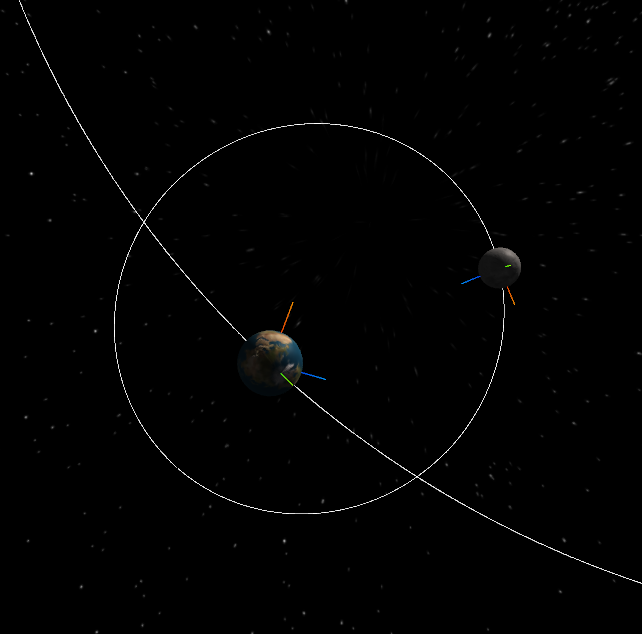
\includegraphics[width=\textwidth]{images/earthandmoonaxisspinabove1}
                \caption{The Earth and Moon spinning on their own axes}
                \label{fig: The axial spin of the Earth and moon.}
       \end{subfigure}
        \begin{subfigure}[b]{0.4\textwidth}
                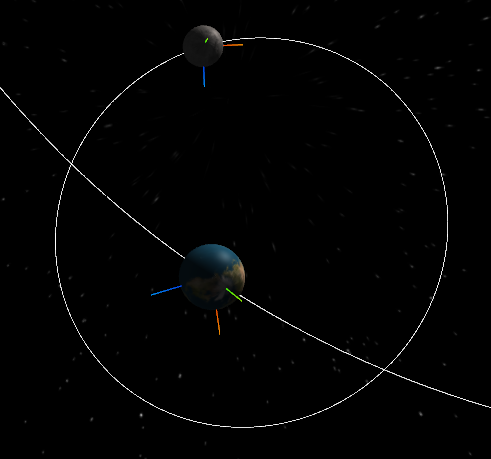
\includegraphics[width=\textwidth]{images/earthandmoonaxisspinabove2}
                \caption{The Earth and Moon spinning on their own axes}
                \label{fig: The axial spin of the Earth and moon.}
       \end{subfigure}
               \begin{subfigure}[b]{0.4\textwidth}
                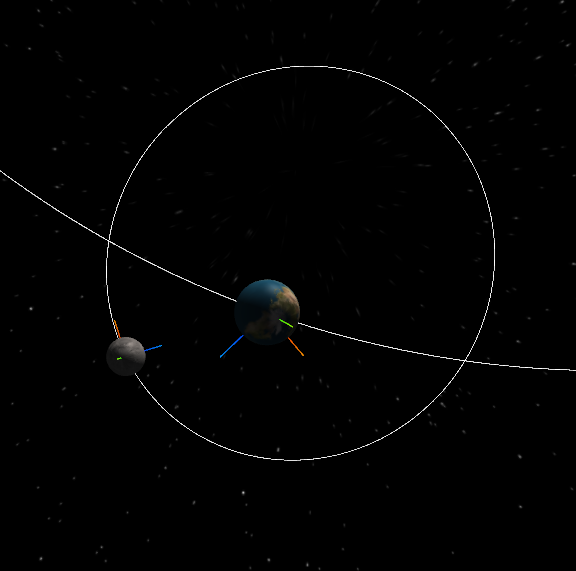
\includegraphics[width=\textwidth]{images/earthandmoonaxisspinabove3}
                \caption{The Earth and Moon spinning on their own axes}
                \label{fig: The axial spin of the Earth and moon.}
       \end{subfigure}
               \begin{subfigure}[b]{0.4\textwidth}
                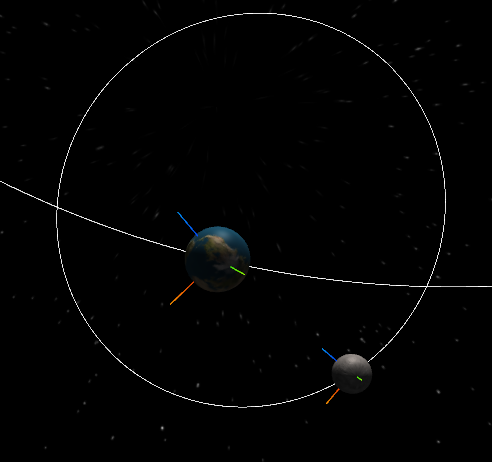
\includegraphics[width=\textwidth]{images/earthandmoonaxisspinabove4}
                \caption{The Earth and Moon spinning on their own axes}
                \label{fig: The axial spin of the Earth and moon.}
       \end{subfigure}
       \caption{Collections of images to present the Moon spinning on its own axis.}\label{fig: The Moon's axial rotation.}
\end{figure}

\subsection{The sun shown as a self-illuminated sphere}
To present the Sun as a self-illuminated sphere, I first used an emissive map, which lights the texture applied to the Mesh, and then added some Ambient lighting, for the purpose of showing the Sun as if it had it's own light and also to help the viewer see the backs of the planets somewhat too. Additionally, I thought it looked good to have a glowing effect around the Sun. I achieved this using the technique by using examples from Lee Stemkoski\cite{sunglow}. I created two glow effects, one larger than the other, to give the impression of the light being more intense as the viewer looked directly at the Sun. 

\begin{figure}[H]
        \centering
        \begin{subfigure}[b]{0.4\textwidth}
                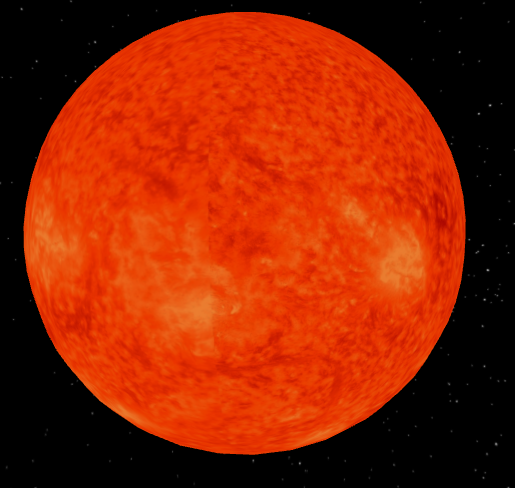
\includegraphics[width=\textwidth]{images/sunemissive}
                \caption{The Sun with just an emissive map for self-illiminating}
                \label{fig:Self-illuminating Sun with emissive map.}
       \end{subfigure}
       %add desired spacing between images, e. g. ~, \quad, \qquad etc.
         %(or a blank line to force the subfigure onto a new line)
        \begin{subfigure}[b]{0.4\textwidth}
                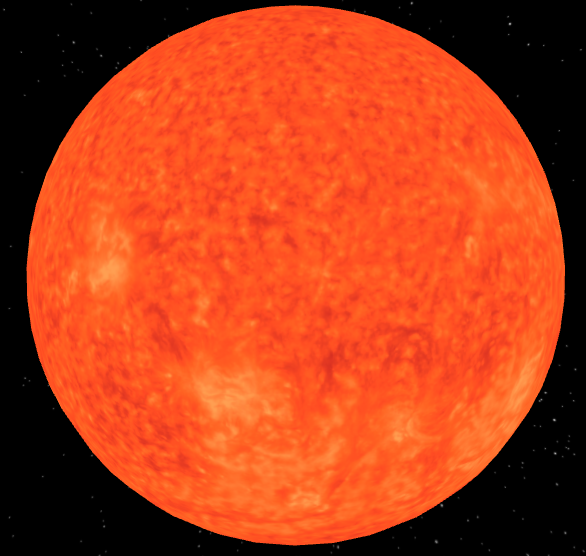
\includegraphics[width=\textwidth]{images/sunemissiveandambient}
                \caption{The Sun with emissive map and ambient lighting.}
                \label{fig:Self-illuminating Sun with emissive map.}
       \end{subfigure}
        \begin{subfigure}[b]{0.4\textwidth}
                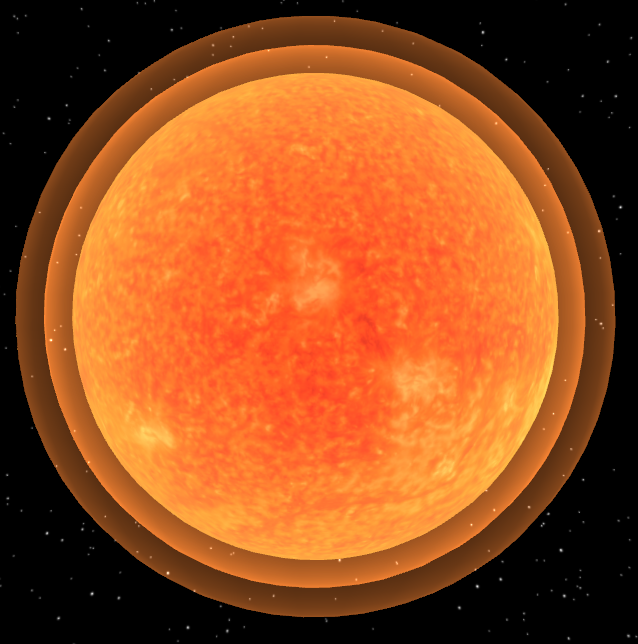
\includegraphics[width=\textwidth]{images/sunwithglow}
                \caption{The Sun with emissive map, ambient lighting and glow effect.}
                \label{fig:Self-illuminating Sun with emissive map.}
       \end{subfigure}
        \caption{The Sun with the three ways it is presented as self-illuminated.}\label{fig:Self-illuminated Sun}
\end{figure}

\subsection{Earth and Moon lit by a single point light source located at the centre of the Sun}
All objects in the scene are lit slightly by a dark AmbientLight for the purpose of the animation. The light source from the Sun is a SpotLight, not a PointLight as requested by the Basic Features. The main reason for this is that Point Lights in three.js do not cast shadows. 

In order to light the Earth and Moon with the Spot Light, I have the light starting at the centre of the Sun (0,0,0) and added as part of the SunMesh for rendering efficiency, and its target set as the position of the Earth, tracking it every animation frame to give the illusion of a single light source at the centre of the Sun.

%----------------------------------------------------------------------------------------
%	Additional Features
%----------------------------------------------------------------------------------------

\section{Additional Features}
\subsection{User Interface}
Shiny UI, look at this picture. You can change speed, move the camera to look at the Sun, Earth or Moon, move the camera around the setting, reset the camera, pause the simulation (pauses the updating of values while still rendering the scene) and turn on or off helpers to visually see the orbital rotations and the axes of the objects. Uses dat.gui \cite{datgui} which makes for quick and easy gui by adding controls and parameters for them, including values and functions.

\begin{figure}[H]
        \centering
        \begin{subfigure}[b]{0.4\textwidth}
                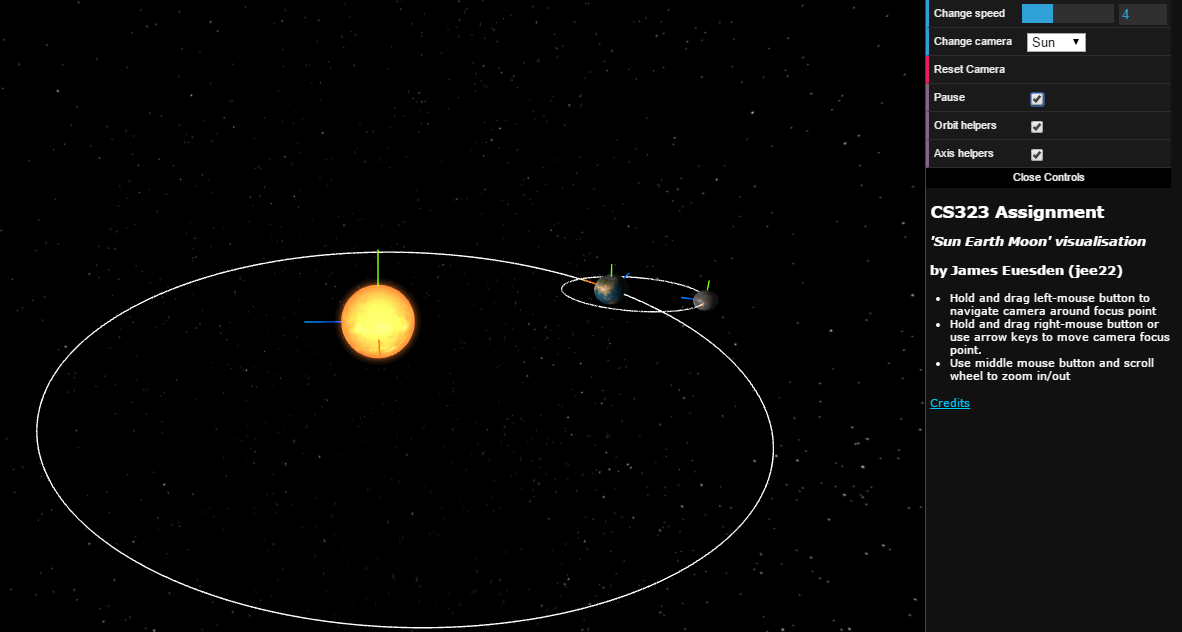
\includegraphics[width=\textwidth]{images/userinterface}
                \caption{The user interface on the page.}
                \label{fig: The user interface.}
	 \end{subfigure}
        \begin{subfigure}[b]{0.4\textwidth}
                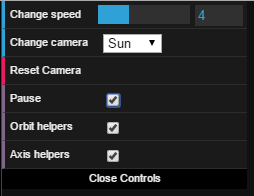
\includegraphics[width=\textwidth]{images/closeupui}
                \caption{The user interface up close.}
                \label{fig: Close up of the user interface.}
	 \end{subfigure}
\end{figure}

\subsection{Synchronous orbital and axial rotation of the Moon}
Well, I did this at first by keeping the speed of the Moon's rotation and it's orbit the same, which worked perfectly. However, when I switched to pre-computing the elliptical orbit, the orbit and rotation no longer matched. I could compute the new rotation by rotating the Moon on the Y axis by the same amount of time steps and speed as the orbit, but I don't believe it would look too accurate, and with the orbital rotation also titled, it would mean calculating how the x and z axis should also be rotated. While possible to do this, for this simple visualisation, I chose to achieve this by using a tool in the three.js library `.lookAt()'. This method updates the rotation of an object to always face the target. In this case, it keeps the synchronus axial and orbital rotation of the moon so the same face is always pointing towards the Earth. Look at this cool set of images that shows the Moon always facing the Earth! Wow!

\subsection{Lighting of the Earth and Moon in Phong shading}
I didn't write my own Phong shader, but here, I used three.js to use Phone Mesh and have used the SpotLight to get Shadows and stuff. Is that enough? Idk what you want from me. Used a specular map to do this cool reflection on the water thing, while the rest absorbs the light better. Shiny.

\subsection{Non-illuminated parts of the Earth and Moon to be shown in shadow}
Due to the dark colour of the ambient light and the light source in the Sun being quite intense, this effect is achieved, see this picture here. Always darker on the side facing away from the Sun. Cool!

\subsection{Constant tilt of the Earth's axis}
Look, see this with Axis Helper. This is super simple to achieve. We just set the Earth's rotation on the z axis to be 23.4 once, when we create it, and it's like that and always in that direction. It spins upon this axis with the transformation matrix to have the correct axial rotation, but the tilt always stays in the one direction, to be a proper representation of the Earth and how it doesn't wobble on it's axis. See here, on each side of the Sun, the axis stays the same direction.

\subsection{Constant tilt of the Moon's orbit}
Here, look, it does this! See in this image, and in this image on the other side of the orbit, the rotation is a constant tilt. This is achieved through the pre-computed points then being multiplied by a rotation on the z axis (could also be the z axis, but this is what I chose) with a transformation matrix. I chose to use three.js applyMatrix4 with my own rotation matrix. I could have written my own Matrix transformation method, as I did for the rotation on the Y axis, however, since this is multiplying a Vector3 by a Matrix4, and I have already shown that I have mastered the command of matrix transformations, I chose to cut down on the amount of code I would need to write for this simple simulation.

\subsection{Elliptical Orbits \& Non-uniform orbital velocities: Kepler's 2nd Law of Planetary Motion}
For both of these additonal points, they tie together. Through calculating one, the other appears. I used the formula provided in the assignment brief \cite{assignment} in order to achieve this, and my code can be seen here: CODE INSERT LOL. This does this: Some cool stuff where we work out the theta for each angle of rotation, using the semi-major axis of the Earth and its distance from the Sun. This is the same for the Earth. You can see how the result looks here, using the Orbital Lines: During testing, I created just the orbital lines to see what the orbit path was like, and changing the number of time steps changed the speed of the orbit (as it was how many points it had to travel along to reach a full cycle) and changing the eccentricity changed how eccentric the ellipse of the orbit was. We can also see that at certain points, the Earth/Moon moves faster where the points are closer, simulating Kepler's 2nd Law of Planetary Motion.

\subsection{Eclipse Shadows}
Through the use of a SpotLight and its shadow camera, turning the ShadowMap of the renderer on, we get this effect: Here, look at some screenshots of it happening. Very easy to achieve. However, previously encountered issues with double shadows, with a WebGL issue that I couldn't fix in my own code. Struggled for a long time with it (others did too, see this link and this link), until an update to three.js fixed it. Relief at fixing it, also frustration at it being something I thought was in my code but turned out not to be. Much time wasted. But it works now, and it's super pretty how it does it with the spot light. Here, you can see my testing with the ShadowCamera, how the shadows are presented within the camera, but not outside of it. COOL!
\begin{lstlisting}
sunLight = new THREE.SpotLight(0xfff0e6, 1, 0);
sunLight.castShadow = true;
sunLight.shadowCameraNear = 20;
sunLight.shadowCameraFar = 190;
sunLight.shadowCameraFov = 45;
// awesome for debugging - Shows the Shadow Camera lines
//scene.add(new THREE.CameraHelper( sunLight.shadow.camera ));
sunLight.target = earthMesh;    
sunLight.position.set(0, 0, 0);
sunMesh.add(sunLight);
\end{lstlisting}

\begin{figure}[H]
        \centering
       
                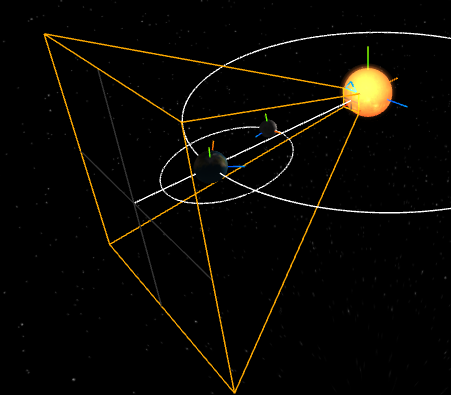
\includegraphics[width=0.5\textwidth]{images/shadowcamera}
                \caption{The Sun light Shadow Camera, showing where shadow casting will be computed.}
                \label{fig: The Shadow Camera.}
      
\end{figure}

You can see the ShadowCamera of the Spot Light in the figure above, as displayed by the ShadowCameraHelper. This helper shows us what the catchment area of the cast shadows will be. Computing where shadows should fall is expensive, and so I've made the shadow camera area small, in order to reduce the cost of computation.

\subsection{Other features of my choice}
Mainly matrix transformations. Previously mentioned them, but I want to express that I wanted to fit them into my assignment. Before I pre-computed the orbits of the Earth and Moon, I was also working on their orbits with matrix transformations, but it became unnecessary once I changed how the orbit was calculated. I still stuck with using matrix transformations for axial rotations, however (where appropriate) and spent some time learning about how to do this. One problem I encountered when working with them was my lighting would not update during an Object's orbit around the light source. This was due to me updating the Geometries vertices but not the face and vertex normals. Once I started updating the Face and Vertex normals (like in three.js own method) see this code here: CODE, it worked as expected. I did test my transformations to check they gave the expected results too (4x4 matrix calculation for each matrix with result HERE PLZ). Many weird attempts with matrix transformations: Working directily with vertices, or working with the Matrix of the object, or working with the Mesh - Flying away Earth, Earth eventually shrinking at the middle (becoming a tube), irregular orbits, etc - Most overcome through looking at the matrix multiply method where I'd inccorectly done the multiplication ordering, or not properly applied the w coordinate on shift translations for the orbital rotations. Happy with the results though.

Sun glow: Just wanted it look cool. While not my own implementation, it was something I felt gave the simulation a little more interest. Code can be found here: SOME CITE. Also cool star map because it looks a little more `real'. Idea for this came from here: CITE LINK.

%--------------------------------------------

%\begin{figure}[H]
%        \centering
%        \begin{subfigure}[b]{0.5\textwidth}
%                \includegraphics[width=\textwidth]{images/compile1}
%                \caption{Cleaning and building}
%                \label{fig:Compile1}
%       \end{subfigure}%
%       ~ %add desired spacing between images, e. g. ~, \quad, \qquad etc.
%         %(or a blank line to force the subfigure onto a new line)
%        \begin{subfigure}[b]{0.5\textwidth}
%                \includegraphics[width=\textwidth]{images/compile2}
%                \caption{Finishing compiling}
%                \label{fig:Compile2}
 %       \end{subfigure}
 %       \caption{Compilation of the program and the output from within the NetBeans IDE on Linux using the 'Clean and Build' function}\label{fig:Compiling the code}
%\end{figure}


%----------------------------------------------------------------------------------------
%	SELF ASSESSMENT
%----------------------------------------------------------------------------------------
\clearpage

\section{Self Assessment}
Here is my self-assessment form, including what has been documented, implemented, whether it can be run, if I referenced all my sources and what grade I would give myself out of 50 (and why that mark in text underneath this neat little table, kthnx).


%----------------------------------------------------------------------------------------
\clearpage

%----------------------------------------------------------------------------------------
%	REFERENCES
%----------------------------------------------------------------------------------------

\begin{thebibliography}{5}

\bibitem{assignment} H. Holstein and Y. Liu, ``A virtual Sun-Earth-Moon system'', CS32310 Advanced Computer Graphics Assignment Semester 1 2015, October 14 2015

\bibitem{xampp} XAMPP Installers and Downloads for Apache Friends, {\em apachefriends}, [online], 

https://www.apachefriends.org/index.html (Accessed 11/06/2015)

\bibitem{earthtextures} Planet Texture Map Collection, {\em planetpixelemporium}, [online],

http://planetpixelemporium.com/planets.html (Accessed 11/06/2015)

\bibitem{suntexture} NASA, {\em NASA}, [online], 

https://www.nasa.gov/sites/default/files/images/700328main\_20121014\_003615\_flat.jpg (Accessed 11/06/2015)

\bibitem{codecolour}  Acknowledgement for code colouring in this report using lstlisting LaTeX: 

javascript - language option supported in listings - TeX - LaTeX Stack Exchange, {\em TeX - LaTeX Stack Exchange}, [online],

<<<<<<< HEAD
  http://tex.stackexchange.com/questions/89574/language-option-supported-in-listings (Accessed: 11/06/2015)
=======
\bibitem{sunglow} Computational Contemplations: Using Shaders and Selective Glow Effects in Three.js, {\em stemkoski}, [online],
http://stemkoski.blogspot.co.uk/2013/03/using-shaders-and-selective-glow.html (Accessed 11/06/2015)

\bibitem{datgui} three.js/dat.gui.min.js at master . mrdoob/three.js, {\em github}, [online],
https://github.com/mrdoob/three.js/blob/master/examples/js/libs/dat.gui.min.js (Accessed 11/06/205)

\bibitem{codecolour}  Acknowledgement for code colouring in this report using lstlisting LaTeX: javascript - language option supported in listings - TeX - LaTeX Stack Exchange, {\em TeX - LaTeX Stack Exchange}, [online], http://tex.stackexchange.com/questions/89574/language-option-supported-in-listings (Accessed: 11/06/2015)
>>>>>>> origin/master

\end{thebibliography}


\end{document}


